\documentclass[../EBEXPaper2.tex]{subfiles}
\begin{document}
%------------------------------------------------- 
\subsubsection{Detector Time Constants}
\label{sec:time_constants}

\begin{itemize}
\item \comred{Write up \ac{LED} tau measurement and data we have (Karl)}
\item \comred{coordinate write-up of other tau measurements e.g. Jeff's, Andrei's.  If we beleive them. (Karl)}
\item \comred{have we talked about loop gain already? I assume so...}
\end{itemize}


The instrinsic time consant of our bolometers, $\tau_0 = C/G \approx 88$~ms \comred{from measured 150 wafer}, 
is defined by the fabrication parameters, see 
Section~\ref{sec:fabrication_parameters}, and describes the thermalization time of the TES to the bath.  
During operation this is modified by the loop gain $\mathcal{L}$ of the TES such that, 
$$\tau_{eff}= \frac{\tau_0}{1+\mathcal{L}}.$$
\cite{aubin_thesis}
Depending on operating conditions, $\tau_{abs}$, the thermalization time of the absorbing spiderweb to the TES, may also be 
important.  From the fabrication parameters of our bolometers, we expect $\tau_{abs} \approx XXX$.  As the bolometer is 
dropped deeper into transition $\mathcal{L}$ increases and $\tau_{eff}$ falls.  Eventually $\tau_{eff} << \tau_{abs}$, and the 
absorber time constant dominates.  To properly characterize our bolometers we need to measure the time constant, which is a 
combination of $\tau_{eff}$ and $\tau_{abs}$, across a range of bias points.  This allows us to disintangle $\tau_{eff}$ and 
$\tau_{abs}$ and determine (\comred{predict a better word?}) the total time constant of our bolometers during flight conditions. We combine direct, 
low noise, lab based measurements of bolometer time constants with noisey, indirect, in-flight measurements to robustly 
determine bolometer time constants during flight. \comred{We don't actually do this yet, but it seems like it may be the plan.
 Unless we just ignore the in flight data.}

We measure time constants in four major ways: response to an electrically chopped \ac{LED} in a test cryostat, Section~\ref{sec:LED_tau}; as part of polarization calibration, Section~\ref{sec:??Polarization??}; \comred{??response to impulsive signals during flight, Section~\ref{sec:??below??}; and from the phase relationship of the 4th and 8th harmonics of the half-wave plate modulated signal, Seciton~\ref{sec:????}.}


\subsubsubsection{LED time-constants}
\label{sec:LED_tau}  

% method, include details of T-bath, \ac{LED} type, chopping, analyzing, etc...

We measure bolometer time constants using the \ac{ETC}.  The \ac{ETC} is a dark cyrostat cooled by 
liquid cryogens to 4~K and to 330~mK by a Helium adsorption refridgerator.  The \ac{ETC} holds a single wafer in a 330~mK light 
tight box which is readout by the same DfMUX and \ac{SQUID} hardware used in flight.  Three \ac{LED}s~\footnote{Fairchild Semiconductor} with 
$\lambda = 940$~nm and $\tau = 1$~$\mu$s are positioned directly above the wafer inside the dark box.  

We measure the time constant by determining the bolometer's response to signals of various frequencies.  The time constant 
acts as a single pole filter, so the bolometer's response will fall as
\begin{equation}
R(f) = \frac{1}{\sqrt{1+(f/f_C)^2}},   % How to label equations?  and what is good format?
\end{equation} \label{eq:single_pole}
where $f$ is the input signal frequency and $f_c$ is the 3~dB cutoff frequency of the bolometer.  The cutoff frequency is 
equivalent to the time constant, $\tau = 1/(2\pi f_c)$.
We electrically chop the \ac{LED}s at a frequency between 0.1 and 80~Hz, using a square wave output by a function generator, and 
record a 2 minute timestream of the bolometer response.  We calculate the power spectrum of this timestream and fit a Fejer 
kernel \citep{Weisse_FejerKernal2006} to the peak centered on the chop frequency to determine power at the chopped 
frequency.  We repeat these measurements at 10 or more chop frequencies and plot response vs chop frequency, 
Figure~\ref{fig:LED_response}.  We determine 
$f_c$ for each detector by fitting equation~\ref{eq:single_pole} to the response data; then convert to $\tau$.  

% need talk of errors.  but not analysed yet.  fejer kernel fit errors?  chi^2 error on single pole fit?
\begin{figure}[ht]
%\epsscale{1.0}
\plotone{images/detectors_and_readout/LED_respons_v_chop}
\caption{Response of bolometer b72w1c2 (how do we reference bolos??) to the \ac{LED} as a function of chop frequency.  Note the 
         characteristic single pole roll-off fit by the dot-dash line.  }
\label{fig:LED_response}
\end{figure}

Figure~\ref{fig:LED_taus} shows the distribution of measured $\tau$ from \ac{EBEX} flight wafer 150-43 at various depths in 
transistion, from $0.98 R_{normal}$ to $0.6 R_{normal}$. \comred{don't restate figure.  need different intro sentence}
This wafer had XXX active bolometers, but we only considered $tau$ values which pass two error cuts.  
The error, $\delta \tau$, was estimated using the fit covarince matrix.  The $tau$ measurement was kept if 
$\delta \tau / \tau > 0.XX$~ms and $\delta \tau < 10$~ms. Roughly XX\% of bolometers failed these criteria, although it 
varied with tuning.  The major reasons for a large $\delta\tau$ were a bolometer latched, so did not respond to the LED, 
or a bolometer was poorly illumated by the LED, so the signal-to-noise was low.
The number of bolometers on 150-43 with measurements of $tau$ ranged from XXX at XX to XXX at XX. This fraction was 
similar for measurements of 250-23 \comred{or just give numbers?}.
For both 150-43 and 250-23 measured $\tau$ qualitatively follows the expectation of $1/(1+\mathcal{L})$; see 
Figure~\ref{fig:taus_vs_Rn}.  \comred{Has Kate talked about loopgain at all?}  

\begin{figure}[ht]
%\epsscale{1.0}
\center
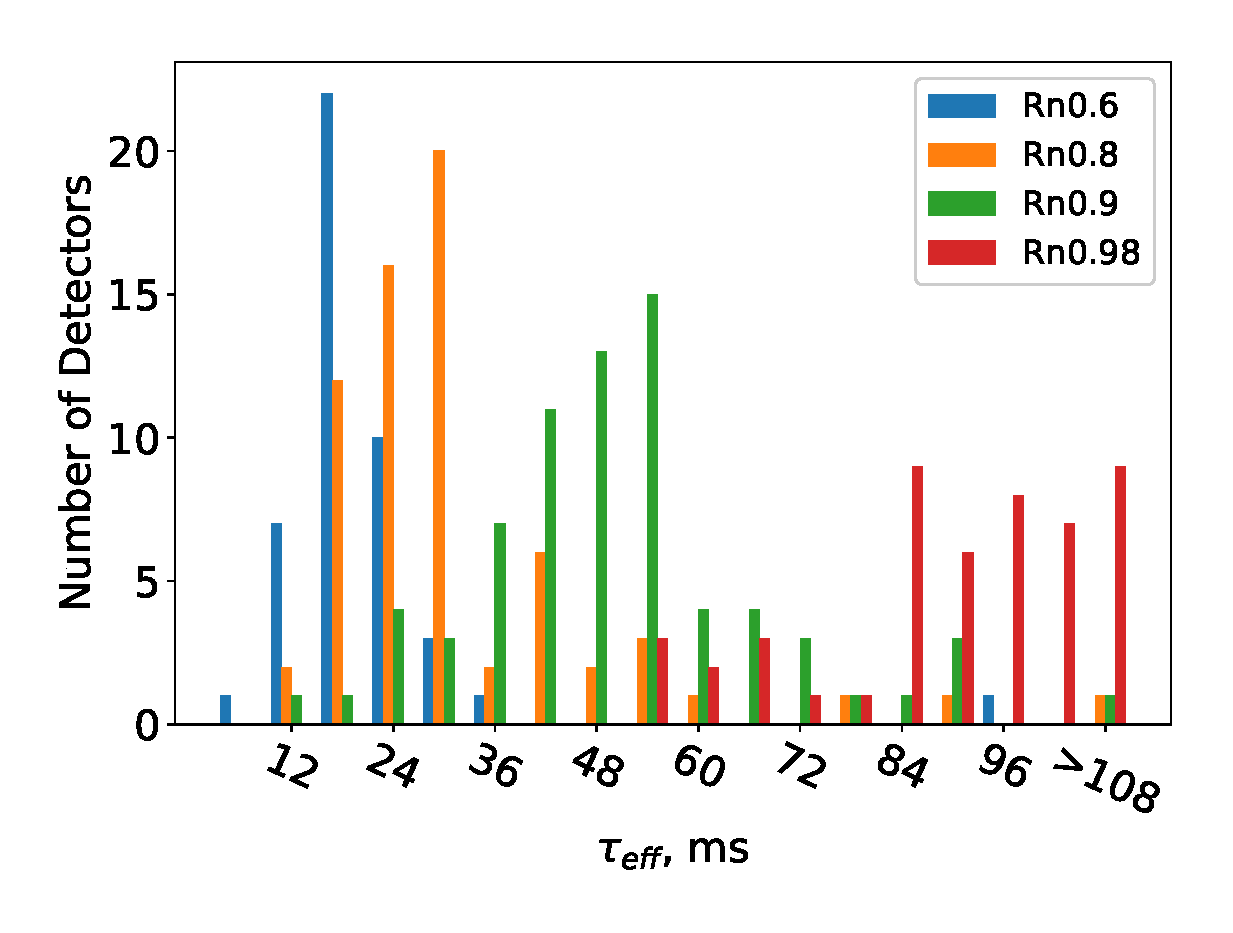
\includegraphics[width=0.48\textwidth]{images/detectors_and_readout/tau_histograms}
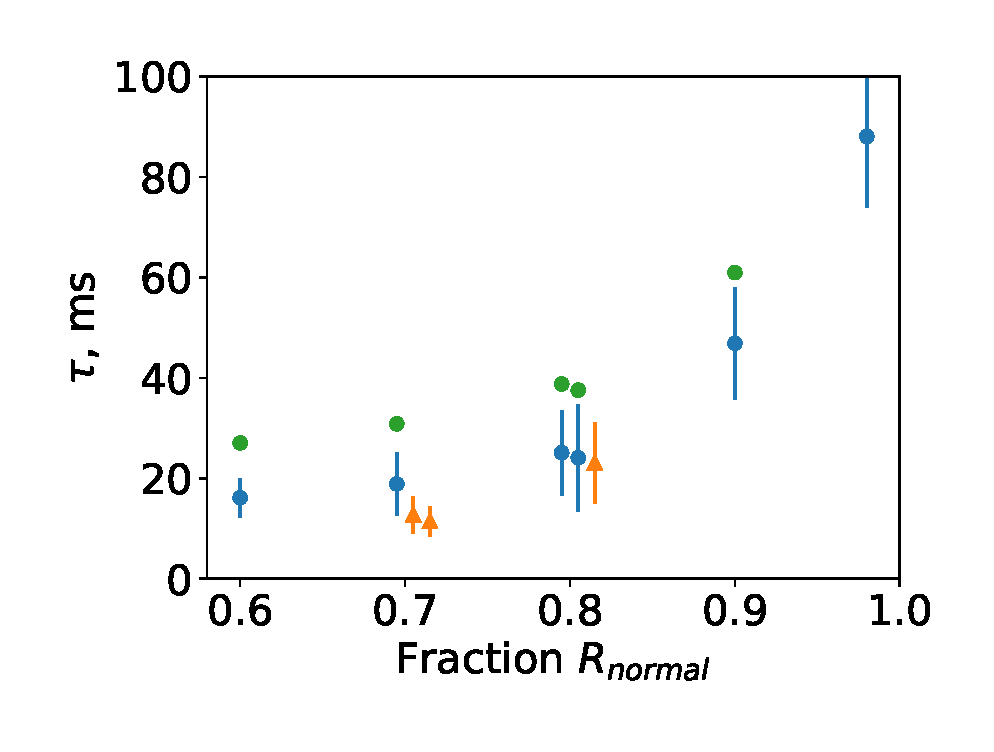
\includegraphics[width=0.48\textwidth]{images/detectors_and_readout/tau_vs_Rn_median}
\caption{Measured $\tau_{eff}$ on wafer 150-43 at various bias points.  For clarity, only a selection of measured transistion 
         depths are shown. \comred{points, speeds up in transition, broad distribution}
         Measured median $\tau_{eff}$ as a function of depth in transition.  Errorbars represent the 1$\sigma$ 
         range for each depth.  Circles are lab \ac{ETC} measurements, triangles are estimates for \ac{EBEX} at 
         float, blue is 150~GHz, and green is 250~GHz. \comred{Colors wrong.  points, speeds up in transition, broad distribution.  same points as above, do 
         we need both?  could add 250's to this plot. }
         }
\label{fig:LED_taus}
\end{figure}

For \ac{EBEX} data analysis we needed $\tau$ at float~\citep{EP1}.  This time constant was not, and was not expected to be, the 
same as what was measured in the lab.  The lower bath temperature of \ac{EBEX}, 250~mK vs 320~mK in the \ac{ETC} changes the 
thermal conductivity, G, of the bolometer to the bath.  Additionally, there is an optical load, which reduces the loopgain. 
Both effects lengthen the time constant.  Following \citet{Hannes_thesis} and using measured bolometer parameters, 
Section~\ref{sec:bolo_char}, we estimate $\tau$ at float to be approximately 1.5 times longer than that measured in the lab. 
Estimates for each wafer and bias point are shown in Figure~\ref{fig:taus_vs_Rn}.  \ac{EBEX} bolometers were typically tuned 
to $85\% R_{normal}$ during flight, so our estimated median $\tau$ is XX~ms.

%\begin{figure}
%%\epsscale{1.0}
%\plotone{images/detectors_and_readout/tau_vs_Rn_median}
%\caption{Measured median $\tau_{eff}$ as a function of depth in transition.  Errorbars represent the 1$\sigma$ 
%         range for each depth.  Circles are lab \ac{ETC} measurements, triangles are estimates for \ac{EBEX} at 
%         float, blue is 150~GHz, and green is 250~GHz. \comred{points, speeds up in transition, broad distribution.  same points as above, do 
%         we need both?  could add 250's to this plot. }}
%\label{fig:taus_vs_Rn}
%\end{figure}



\comred{Plan is to add a histogram of taus.  Maybe useful?  Other possible plots:  \\ 
PSD with fit.  \\
response vs chop frequency (almost certainly) \\
some representation of tau changing with \%Rn .}

\comred{After we see the data...  Comments on tau vs depth in transition.  And does $\tau_{eff}$ or $\tau_{abs}$ domintate? \\
  Also talk about errors.}

\comred{Compare with ETF measurements?  what exist? Jeff's data?}


%HAve data for 250-23 (Karl)  2 or 3 depths
%and 150-15 (Kate, May 2011). ?? depths
%and 150-43  many depths and 1.

%------------------------------------------------
%\include{DetectorReadoutBibliography}
\end{document}